\newcommand{\thetm}{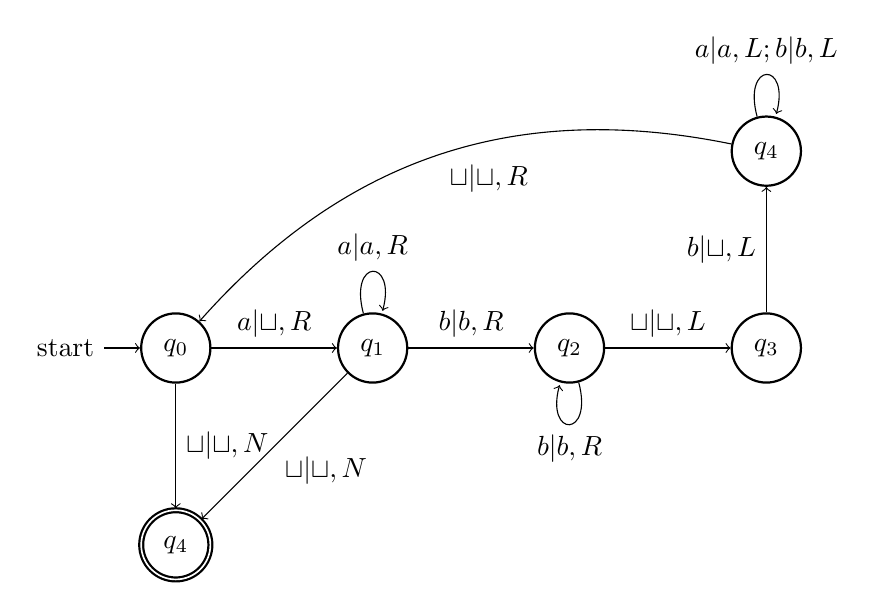
\begin{tikzpicture}[node distance=2.5cm,auto]
  \node(q0)[state,initial]{$q_0$};
  \node(q1)[state,right of=q0]{$q_1$};
  \node(q2)[state,right of=q1]{$q_2$};
  \node(q3)[state,right of=q2]{$q_3$};
  \node(q4)[state,above of=q3]{$q_4$};
  \node(q5)[state,accepting,below of=q0]{$q_4$};
  \path[->]       (q0) edge node{$a|\sqcup,R$} (q1)
	          (q0) edge node{$\sqcup|\sqcup,N$} (q5)
	          (q1) edge[loop above] node{$a|a,R$} ()
	          (q1) edge node{$b|b,R$} (q2)
	          (q1) edge node{$\sqcup|\sqcup,N$} (q5)
	          (q2) edge[loop below] node{$b|b,R$} ()
	          (q2) edge node{$\sqcup|\sqcup,L$} (q3)
	          (q3) edge node{$b|\sqcup,L$} (q4)
	          (q4) edge[loop above] node{$a|a,L; b|b,L$} ()
	          (q4) edge[bend right] node{$\sqcup|\sqcup,R$} (q0);
 \end{tikzpicture}}

\documentclass[t]{beamer}
\usetheme[deutsch]{KIT}
\setbeamercovered{transparent}
\setbeamertemplate{navigation symbols}{}

\KITfoot{Tutoriumsmaterial von Joachim Priesner, Sebastian Ullrich und Max Wagner \hspace{2.5cm} Basierend auf den Folien von Simon Stroh und Moritz v. Looz}
\usepackage[utf8]{inputenc}
\usepackage{amsmath}
\usepackage{ifthen}
\usepackage{amssymb}
\usepackage{tikz}
\usepackage{ngerman}
\usetikzlibrary{automata}
\usenavigationsymbols


\title{Theoretische Grundlagen der Informatik}
\subtitle{Tutorium}
\author{Moritz von Looz, Simon Stroh}

\institute[ITI]{Institut für Theoretische Informatik}

\TitleImage[height=\titleimageht]{images/tmaschine.png}

\newcommand{\N}{\ensuremath{\mathbb{N}}}
\newcommand{\M}{\ensuremath{\mathcal{M}}}
\newcommand{\classP}{\ensuremath{\mathcal{P}}}
\newcommand{\classNP}{\ensuremath{\mathcal{NP}}}
\newcommand{\co}{\ensuremath{\mathsf{co\text{-}}}}
\newcommand{\pot}{\ensuremath{\mathcal{P}}}
\newcommand{\abs}[1]{\ensuremath{\left\vert #1 \right\vert}}
\newcommand{\menge}[2]{\ensuremath{\left\lbrace #1 \,\middle\vert\, #2 \right\rbrace}}
\newcommand{\ducttape}[1]{\vspace{#1}}
\newcommand{\neglit}[1]{\overline{#1\vphantom{x^a}}}
\newcommand{\recipe}{\raisebox{-.3cm}{
\includegraphics[scale=.15]{images/chefs-cap.png}}\hspace{0.2cm}}

\newcommand{\invincible}{\setbeamercovered{invisible}} %  "Yesss! I am invincible!!" (Boris Grishenko)
\newcommand{\vincible}{\setbeamercovered{transparent}}

% \@ifundefined{tikzset}{}{\tikzset{initial text=}} % Text "start" bei Startknoten unterdrücken
\tikzstyle{every node}=[thick]
\tikzstyle{every line}=[thick]

\newcommand{\tutnr}[1]{
  \subtitle{Tutorium #1}
	\begin{frame}
		\maketitle
	\end{frame}
}

\newcommand{\uebnr}[1]{
  \subtitle{Anmerkungen zum #1. Übungsblatt}
	\begin{frame}
		\maketitle
	\end{frame}
}

\begin{document}

\tutnr{4}

\section{Wdh: Nerode-Relation}
\begin{frame}
	\frametitle{Aufgabe zur Nerode-Relation}
	
	Sei $\Sigma = \{a\}$.
Zeigen Sie mit Hilfe der Nerode-Relation die Nichtregularit\"at der Sprache $L$: 

\[L := \{w \in \Sigma^*\mid w = a^{n^2},\; n \in \N\}.\]
\end{frame}

\section{Entscheidbarkeit}
\begin{frame}
 \frametitle{Definitionen zur TM (Vorlesung)}
 \begin{enumerate}
  \item Eine TM \emph{akzeptiert} eine Eingabe $w \in \Sigma^*$, wenn sie nach Lesen von $w$ in einem Zustand aus $F$ stoppt.
  \item Sie \emph{akzeptiert} eine Sprache $L \subseteq \Sigma^*$, wenn sie genau die Wörter $w$ aus $L$ als Eingabe akzeptiert.
\end{enumerate}
\end{frame}
\begin{frame}
 \frametitle{Definitionen zur TM (Vorlesung)}
 \begin{enumerate}
 \setcounter{enumi}{2}
 \item Eine Sprache $L \subseteq \Sigma^*$ heißt \emph{rekursiv} oder \emph{entscheidbar}, wenn es eine Turingmaschine gibt, die auf allen Eingaben stoppt und
	ein Wort $w \in \Sigma^*$ genau dann akzeptiert, wenn $w \in L$ gilt.
  \item Eine Sprache $L \subseteq \Sigma^*$ heißt \emph{rekursiv-aufzählbar} oder \emph{semi-entscheidbar}, wenn es eine Turingmaschine gibt, 
	die genau $w$ genau dann akzeptiert, wenn $w \in L$ gilt. \\ Das Verhalten der Turingmaschine für Eingaben $w \not\in L$ ist damit nicht definiert.
	Sie stoppt entweder nicht in einem Endzustand oder aber stoppt gar nicht.
	\item Eine TM \emph{realisiert} die Funktion $f: \Sigma^* \rightarrow \Gamma^*$ mit $$f(w) = \begin{cases} \text{Ausgabe der TM nach Abarbeitung von } w & \text{wenn die TM hält} \\ \text{undefiniert} & \text{sonst} \end{cases}$$
 \end{enumerate}
\end{frame}

\begin{frame}
 \frametitle{Beispiel zur Akzeptanz}
 \begin{itemize}
  \item $\Sigma := \{a, b\}$  
  \item $F := \{q_4\}$
  
  \ducttape{-1cm} 
  \thetm
 \end{itemize}
 
 \end{frame}

\begin{frame}
 \frametitle{Sprache}
 \begin{itemize}
  \item $aab$ wird von der TM akzeptiert.
  \item $abb$ nicht.
  \item Die akzeptierte Sprache ist $L(TM) := \menge{a^kb^l}{k \geq l}$
 

 \hfill 
 \resizebox{8cm}{!} {%
  \thetm
 }
  \invincible
  \pause
 \ducttape{-6cm} 
  \item ist diese Sprache semi-entscheidbar?
  \pause
  \item Ist sie auch entscheidbar?
  \vincible
 \end{itemize}
 
\end{frame}


%TODO Beispiel für nicht entscheidbare Probleme
%TODO Beispiel für Entscheidbarkeit

\section{Universelle Turingmaschine}
\begin{frame}
\frametitle{Universelle Turingmaschine}
\begin{block}{Gödelnummer}
\begin{itemize}
\item Jede TM lässt sich eindeutig als Zahl, ihre \emph{Gödelnummer}, kodieren.
\item Ungültige Gödelnummer $\cong$ TM, die alle Eingaben ablehnt.
\end{itemize}
\end{block}
\begin{block}{Universelle Turingmaschine}
\begin{itemize}

\item Eingabe:
\begin{enumerate}
\item Kodierung einer TM
\item Eingabe für die zu simulierende TM
\end{enumerate}
\item Simulation der übergebenen TM
\item Ausgabe: Ausgabe der simulierten TM.
\end{itemize}
\end{block}
\end{frame}


\begin{frame}
\frametitle{Aufgaben zur Entscheidbarkeit}
\begin{itemize}
\item Seien $L_1$ und $L_2$ zwei Sprachen über einem Alphabet $\Sigma$.
Beweisen Sie:
\begin{enumerate}
\item Ist $L_1$ entscheidbar, so ist auch $L_1^c$ entscheidbar.
\item Sind $L_1$ und $L_2$ entscheidbar, so ist auch $L_1\cup L_2$ entscheidbar.
\item Sind $L_1$ und $L_2$ entscheidbar, so ist auch $L_1\setminus L_2$ entscheidbar.
\item Ist $L_1$ entscheidbar, so ist auch die Sprache 
$$\min(L_1):=\menge{x\in L_1}{\text{kein echtes Präfix von $x$ ist in }L_1}$$
entscheidbar.
\end{enumerate}
\item Ist die Sprache der Busy-Beaver-Turingmaschinen mit maximal 42 Zuständen entscheidbar?
\end{itemize}
\end{frame}

\begin{frame}
 \frametitle{Aufgabe zur Semi-Entscheidbarkeit}
Sei $L$ eine semi-entscheidbare Sprache, die nicht entscheidbar ist. Ist die
Sprache $L'=\{0w \mid w \in L\} \cup \{1w \mid w \not\in L\}$ entscheidbar,
semi-entscheidbar oder keins von beiden?

Hinweis: Nimm an, $L'$ sei semi-entscheidbar, und folgere daraus, dass
dann $L$ entscheidbar ist. 
\end{frame}

\begin{frame}
   \frametitle{Aufgabe}
	\begin{enumerate}
\item Zeige, dass die Sprache $L_{\emptyset} := \{\langle \mathcal M \rangle \mid \mathcal M \text{ Turingmaschine}, L(\mathcal M) = \emptyset\}$ nicht entscheidbar ist.
\item Zeige, dass die Komplementsprache $L_{\emptyset}^c$ zu $L_{\emptyset}$ \emph{semi-}entscheidbar ist.
\end{enumerate}
\end{frame}


\begin{frame}
 \frametitle{Halteproblem}
 Zeige, dass das Halteproblem semi-entscheidbar ist.
\end{frame}

\section{Erweiterungen von Turingmaschinen}
\begin{frame}
\frametitle{Erweiterungen von Turingmaschinen}
\begin{block}{Erweiterungen}
Es gibt mehrere zu Turingmaschinen (bezüglich Berechenbarkeit) äquivalente Berechnungsmodelle, die der Turingmaschine sehr ähnlich sind. Man spricht hier von Erweiterungen von Turingmaschinen. Diese verwendet man gerne in Beweisen, da sie oft übersichtlicher sind.
\end{block}
\end{frame}
% Mehrkopf
\begin{frame}
\frametitle{Mehrkopf-Turingmaschinen}
\begin{figure}[H]
\begin{center}
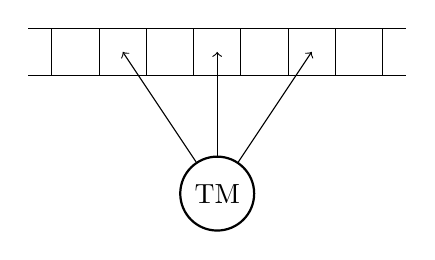
\begin{tikzpicture}[scale=0.3]
\draw (-8,1) -- (8,1);
\draw (-8,-1) -- (8,-1);
\draw (7,1) -- (7,-1);
\draw (5,1) -- (5,-1);
\draw (3,1) -- (3,-1);
\draw (1,1) -- (1,-1);
\draw (-1,1) -- (-1,-1);
\draw (-3,1) -- (-3,-1);
\draw (-5,1) -- (-5,-1);
\draw (-7,1) -- (-7,-1);
\node[draw,circle] (tm) at (0,-6) {TM};
\draw[->] (tm) -- (0,0);
\draw[->,bend left] (tm) -- (-4,0);
\draw[->,bend right] (tm) -- (4,0);
\end{tikzpicture}
\end{center}
\end{figure}
Eine Mehrkopf-Turingmaschine hat mehrere Lese-/Schreibeköpfe. Die Zustandsänderung hängt nun von dem gelesenen Zeichen aller Köpfe ab und kann auch alle Köpfe verschieben bzw. mit allen gleichzeitig schreiben.
\begin{block}{Änderungen in der Definition}
$$ \delta: Q \times \Gamma^n \rightarrow Q \times \Gamma^n \times \{L,N,R\}^n$$
\end{block}
\end{frame}

% Mehrband
\begin{frame}
\frametitle{Mehrband-Turingmaschinen}
\begin{figure}[H]
\begin{center}
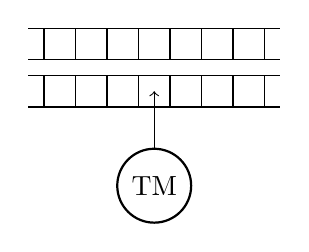
\begin{tikzpicture}[scale=0.2]
\draw (-8,4) -- (8,4);
\draw (-8,2) -- (8,2);
\draw (7,4) -- (7,2);
\draw (5,4) -- (5,2);
\draw (3,4) -- (3,2);
\draw (1,4) -- (1,2);
\draw (-1,4) -- (-1,2);
\draw (-3,4) -- (-3,2);
\draw (-5,4) -- (-5,2);
\draw (-7,4) -- (-7,2);

\draw (-8,1) -- (8,1);
\draw (-8,-1) -- (8,-1);
\draw (7,1) -- (7,-1);
\draw (5,1) -- (5,-1);
\draw (3,1) -- (3,-1);
\draw (1,1) -- (1,-1);
\draw (-1,1) -- (-1,-1);
\draw (-3,1) -- (-3,-1);
\draw (-5,1) -- (-5,-1);
\draw (-7,1) -- (-7,-1);

\draw (-8,1) -- (8,1);
\draw (-8,-1) -- (8,-1);
\draw (7,1) -- (7,-1);
\draw (5,1) -- (5,-1);
\draw (3,1) -- (3,-1);
\draw (1,1) -- (1,-1);
\draw (-1,1) -- (-1,-1);
\draw (-3,1) -- (-3,-1);
\draw (-5,1) -- (-5,-1);
\draw (-7,1) -- (-7,-1);
\node[draw,circle] (tm) at (0,-6) {TM};
\draw[->] (tm) -- (0,0);
\end{tikzpicture}
\end{center}
\end{figure}
Eine Mehrband-Turingmaschine hat mehrere Bänder. Die Zustandsänderung kann nun auch auf ein anderes Band wechseln. Dabei wird immer auf die zuletzt eingenommene Position auf dem anderen Band gewechselt 
\begin{block}{Änderungen in der Definition}
$$ \delta: Q \times \Gamma \times \{1, \ldots, n\} \rightarrow Q \times \Gamma \times \{L,N,R\} \times \{1, \ldots, n\}$$
\end{block}
\end{frame}
% Mehrdim
\begin{frame}
\frametitle{Mehrdimensionale Turingmaschinen}
\begin{figure}[H]
\begin{center}
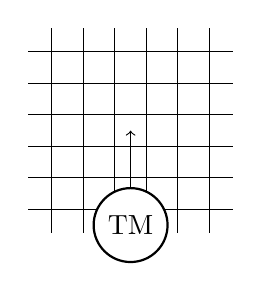
\begin{tikzpicture}[scale=0.2]
\draw[step=2cm,xshift=1cm,yshift=1cm] (-7.5,-7.5) grid (5.5,5.5);
\node[draw,circle,fill=white] (tm) at (0,-6) {TM};
\draw[->] (tm) -- (0,0);
\end{tikzpicture}
\end{center}
\end{figure}
Eine mehrdimensionale Turingmaschine hat ein mehrdimensionales Band, der Kopf kann sich dann in allen verfügbaren Dimensionen bewegen.
\begin{block}{Änderungen in der Definition (für Dimension 2)}
$$ \delta: Q \times \Gamma \rightarrow Q \times \Gamma \times \{L,N,R,U,D\}$$
\end{block}
\end{frame}

\section{Satz von Rice}
\begin{frame}
\frametitle{Satz von Rice}
Der Satz von Rice sagt aus, dass es unmöglich ist, eine nichttriviale Eigenschaft von Turingmaschinen algorithmisch zu entscheiden.
\begin{block}{Formale Version}
Es sei $R$ die Klasse aller Turing-berechenbaren Funktionen und $S$ eine beliebige nichttriviale (das bedeutet $S \neq \emptyset$ und $S \neq R$) Teilmenge davon. Dann ist die Sprache
$$ C_S = \{ i |\text{ die von $M_i$ berechnete Funktion liegt in $S$} \} $$
unentscheidbar. 
\end{block}
\end{frame}
% Beispiel
%\begin{frame}
%\frametitle{Beispiel}
%Die Klasse aller Programme, die etwas auf einem Rechner tun, das der Benutzer nicht möchte (das ist eine Teilmenge der turing-berechenbaren Funktionen) ist unentscheidbar. Daraus folgt, dass es keinen perfekten Virenscanner geben kann!
%\end{frame}

% Aufgabe
\begin{frame}
\frametitle{Aufgabe}
Kann man die Entscheidbarkeit der folgenden Mengen mithilfe des Satzes von Rice bestimmen?
\begin{itemize}
\item Alle Turingmaschinen, die nur $0$ aufs Band schreiben.
\item Alle Turingmaschinen, die im ersten Schritt genau eine $0$ aufs Band schreiben und im zweiten Schritt anhalten. 
\item Alle Turingmaschinen, die überhaupt etwas auf das Band schreiben.
\end{itemize}
\end{frame}

\section{Postsches Korrespondenzproblem}
\begin{frame}
\frametitle{Postsches Korrespondenzproblem}
Gegeben sei eine Folge $P$ von Paaren $((x_1, y_1), (x_2, y_2), \ldots, (x_n,y_n))$ von nichtleeren Worten über einem endlichen Alphabet. Dies nennt man eine \textbf{Instanz} des PKP.
Eine nichtleere Folge $I = i_1, i_2, \ldots, i_m$ von Indizes aus $\{1, \ldots, n\}$ heißt Lösung zu $P$, wenn $x_{i_1}x_{i_2}\ldots{}x_{i_m} = y_{i_1}y_{i_2}\ldots{}y_{i_m}$.
\begin{block}{Beispiel}
\begin{displaymath}
( {a \choose aba}, {ab \choose bb}, {baa \choose aa} )
\end{displaymath}

Lösung: $1,3,2,3$
\begin{displaymath}
{a \choose aba}, {baa \choose aa}, {ab \choose bb}, {baa \choose aa}
\end{displaymath}

\end{block}
\end{frame}

\begin{frame}
\frametitle{Aufgabe}
\begin{enumerate}
\item Finde eine Lösung für folgende Instanz des Post'schen Korrespondenzproblems: 
\[ ((aa, a), (b, aa), (a, aab)) \]
  \item Zeigen Sie, dass folgende Instanz des Post'schen Korrespondenzproblems
        keine Lösung hat:

        \[ ((ab, b), (bba, abb), (ab, ba), (a, abb)) \]

  \item Zeigen Sie, dass das Post'sche Korrespondenzproblem für Wörter
über einem Alphabet mit nur einem Symbol entscheidbar ist.
\end{enumerate}
\end{frame}

\begin{frame}
\frametitle{Aufgabe}
Finde eine Lösung für folgende Instanz des PKP:
$$ ((001,0),(01,011),(01,101),(10,001)) $$

\setbeamercovered{invisible}
\pause

Eine kürzeste Lösung hat mindestens die Länge 66, z.B:
\begin{center}
$ I_1 = $(2,4,3,4,4,2,1,2,4,3,4,3,4,4,3,4,4,2,1,4,\\
4,2,1,3,4,1,1,3,4,4,4,2,1,2,1,1,1,3,4,3,4,1,2,\\
1,4,4,2,1,4,1,1,3,4,1,1,3,1,1,3,1,2,1,4,1,1,3)
\end{center}

\pause


\includegraphics{images/trollface}

\end{frame}

\begin{frame}
	\frametitle{Bis zum nächsten Mal!}
    \begin{center}
        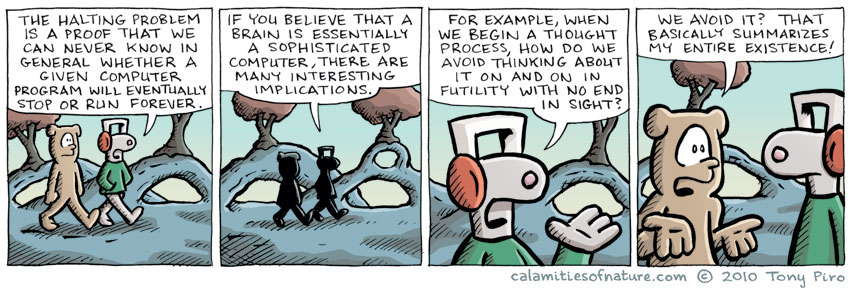
\includegraphics[width=\textwidth]{images/halting.jpg}
    \end{center}
\end{frame}

\frame{
  \frametitle{Lizenzen}
  \center
  \includegraphics[width=2em]{images/by}
  \includegraphics[width=2em]{images/cc}
  \includegraphics[width=2em]{images/sa}
  \\
  {\tiny

Dieses Werk ist unter einem ``Creative Commons Namensnennung-Weitergabe unter gleichen Bedingungen 3.0 Deutschland``-Lizenzvertrag lizenziert. Um eine Kopie der Lizenz zu erhalten, gehen Sie bitte zu \href{http://creativecommons.org/licenses/by-sa/3.0/de/}{http://creativecommons.org/licenses/by-sa/3.0/de/} oder schreiben Sie an Creative Commons, 171 Second Street, Suite 300, San Francisco, California 94105, USA.\\
  \vspace{1cm}
  Davon ausgenommen sind das Titelbild, welches aus der März-April 2002 Ausgabe von American Scientist erschienen ist und ohne Erlaubnis verwendet wird, sowie das KIT Beamer Theme. Hierfür gelten die Bestimmungen der jeweiligen Urheber.
  \vspace{1cm}
  \\ 
  }
  %Habe hier die Reihenfolge etwas umgestellt, weil die Formatierung bei mir komisch aussah. 
  %Wenn es bei dir anders ist, kannst du es auch wieder zurückändern, dann haben wir unterschiedliche Kompilieroptionen
}

\end{document}
